\chapter{Pilots}
We conducted two pilots, the first one did not include the implementation of questions of varying difficulty and the second one did. The main objective when implementing this new question generating algorithm was to try and bring the players closer to a 50\% success rate when answering questions
\section{First pilot}
We made Reminisce.me available to the public and asked family and friends to play the game. Over the course of roughly one week people have answered 1227 over the course of 83 games. We had 25 users which brings us to an average of 3.32 games played by user.
\subsection{Selected Questions}
During this trial, people answered 377 order questions, 348 timeline questions, 317 multiple choice questions and 185 geolocation questions. Of those questions 159 order questions, 174 timeline questions, 192 multiple choice questions and 158 geolocation questions were correct.\\
An other interesting statistics is the number of avoided questions. Without taking into account the state of the board, one can see that 407 order questions, 502 timeline questions, 443 multiple choice questions and 142 geolocation questions were not answered. Aside from random factors (such as the position of the board, which questions were locked etc...), this statistics can be explained by two main factors: the fun of playing a certain question type and the perceived difficulty. While there is nothing that can be said about order question (the number of answered ones is close to the number of avoided ones), it seems like people have a tendency to avoid timeline and multiple choice questions and based on the feedback we got from the users, it might be linked to the perceived difficulty. On the other hand the geolocation are picked with a visibly high ratio. The high success rate on this kind of question is probably a good explanation. Figure \ref{fig:p1TotCorrectAvoid} shows a summary of those results.
\begin{figure}
\centering
{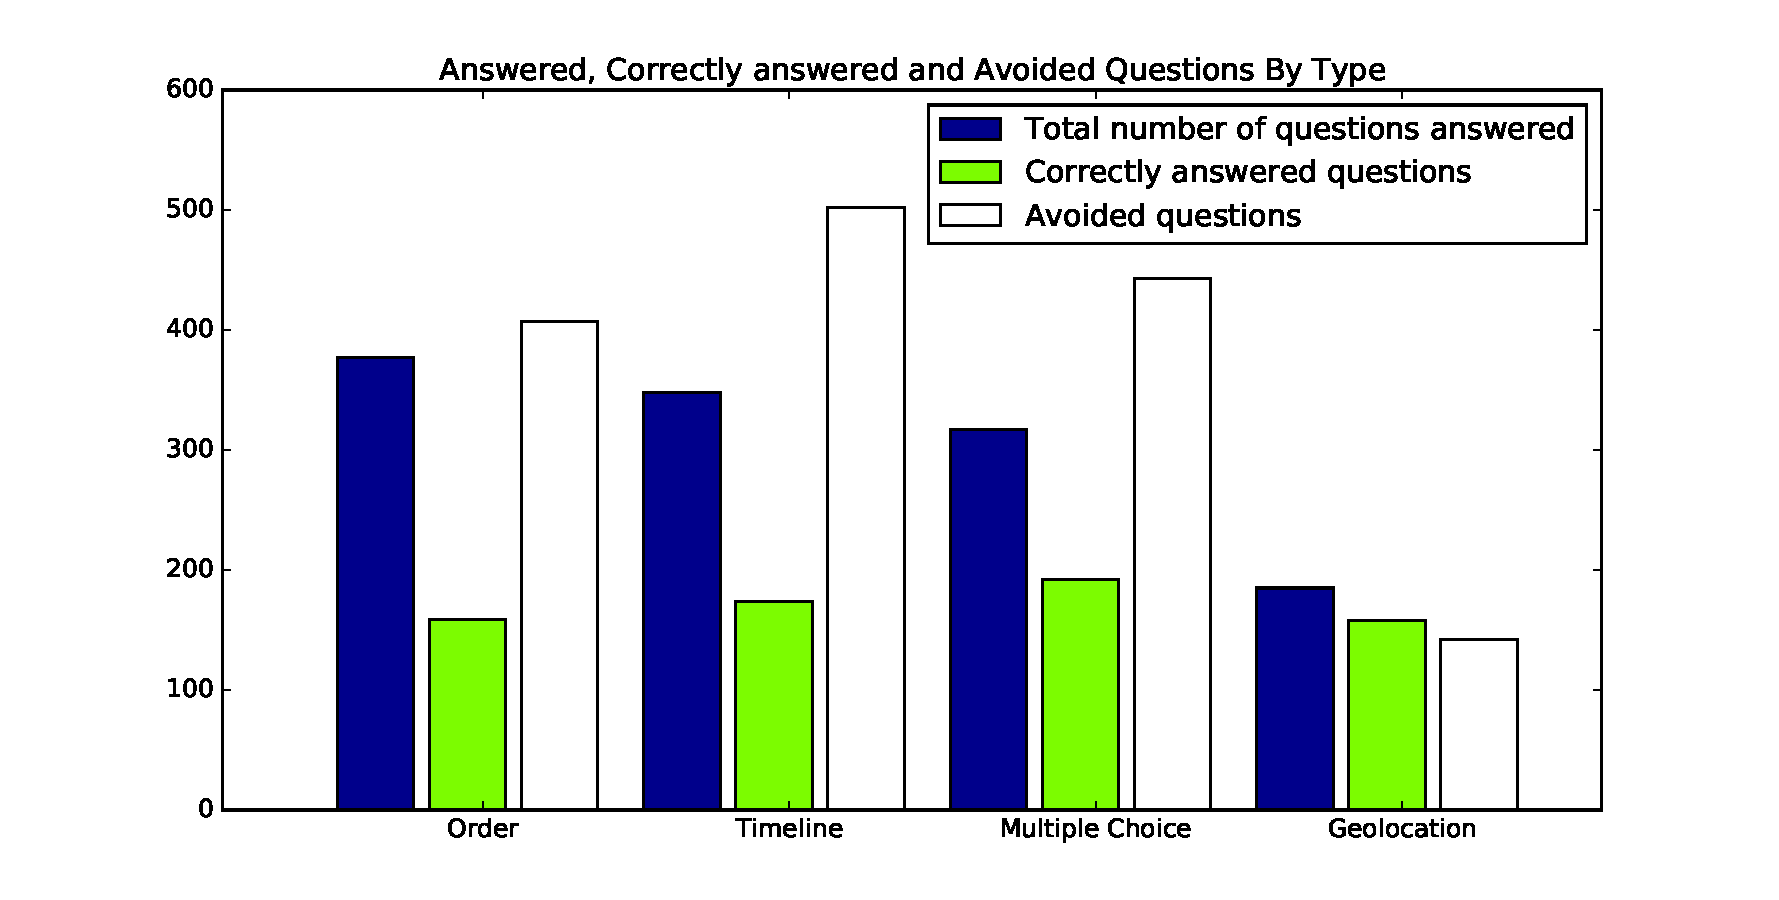
\includegraphics[width=4in]{images/pilot_1_selected_questions.pdf}}
\caption{Total, Correct and Avoided Questions Answered By Type}
\label{fig:p1TotCorrectAvoid}
\end{figure}
\subsection{Remembered Or Randomly Selected}
As for the pilot in June 2016, we can conclude that on average the players tend to try and remember the anwers. The average performance for ordering questions was 35.04\% success rate while when answering at random would yield a 16.67\% success. For timeline we get a 51.07\% success which is more than the 33.33\% random success rate. The result is the same for the multiple choice questions with respectively 58.6\% and 25\% for the measured and random success rate. Finally we measured an extraordinary 61.5\% average success rate on the geolocation. While this last result is impressive it came with a rather high standard deviation and, given the low number of geolocalised posts, the amount of different questions is low and most of the players would be able to learn the answers by heart. Figure \ref{fig:p1Correct} shows a summary of those results.\\
The high variance makes it hard to see how most of the users behaved. The box plot shown on figure \ref{fig:p1Boxes} tells us that for the timeline questions, more than 75\% of users were better than random and that half of the user had between 40\% and 60\% success, which approximatively what we wish to achieve with the difficulty in the second pilot. For order questions, more than half of the participants were better than random but most of the users had a success rate between 15\% and 51\% which is way too low so we would expect the difficulty to improve those results. The multiple choice results give that more than 75\% of the players were better than the random choice and for most of the people the average success rate was between 45\% and 75\%. This is a bit too high and we would expect that the implementation of difficulty would reduce that. When it comes to the geolocation questions we run into some issues, most of the people who had some of them had a success rate between 90\% and 100\%, this corroborates the hypothesis that most of the people who have this kind of question have so few that they can memorize them.
\begin{figure}
\centering
{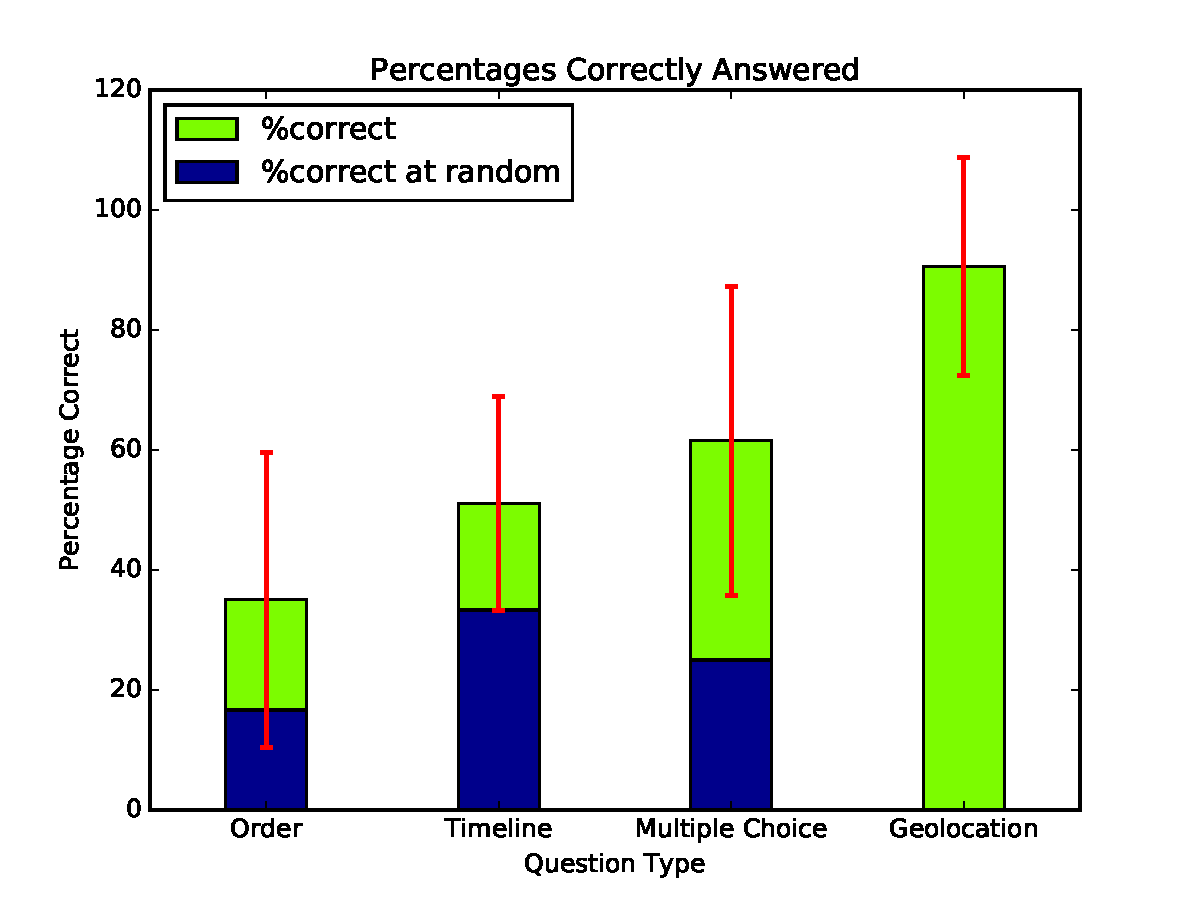
\includegraphics[width=4in]{images/pilot_1_correct.pdf}}
\caption{Percentages Correctly Answered}
\label{fig:p1Correct}
\end{figure}
\begin{figure}
\centering
{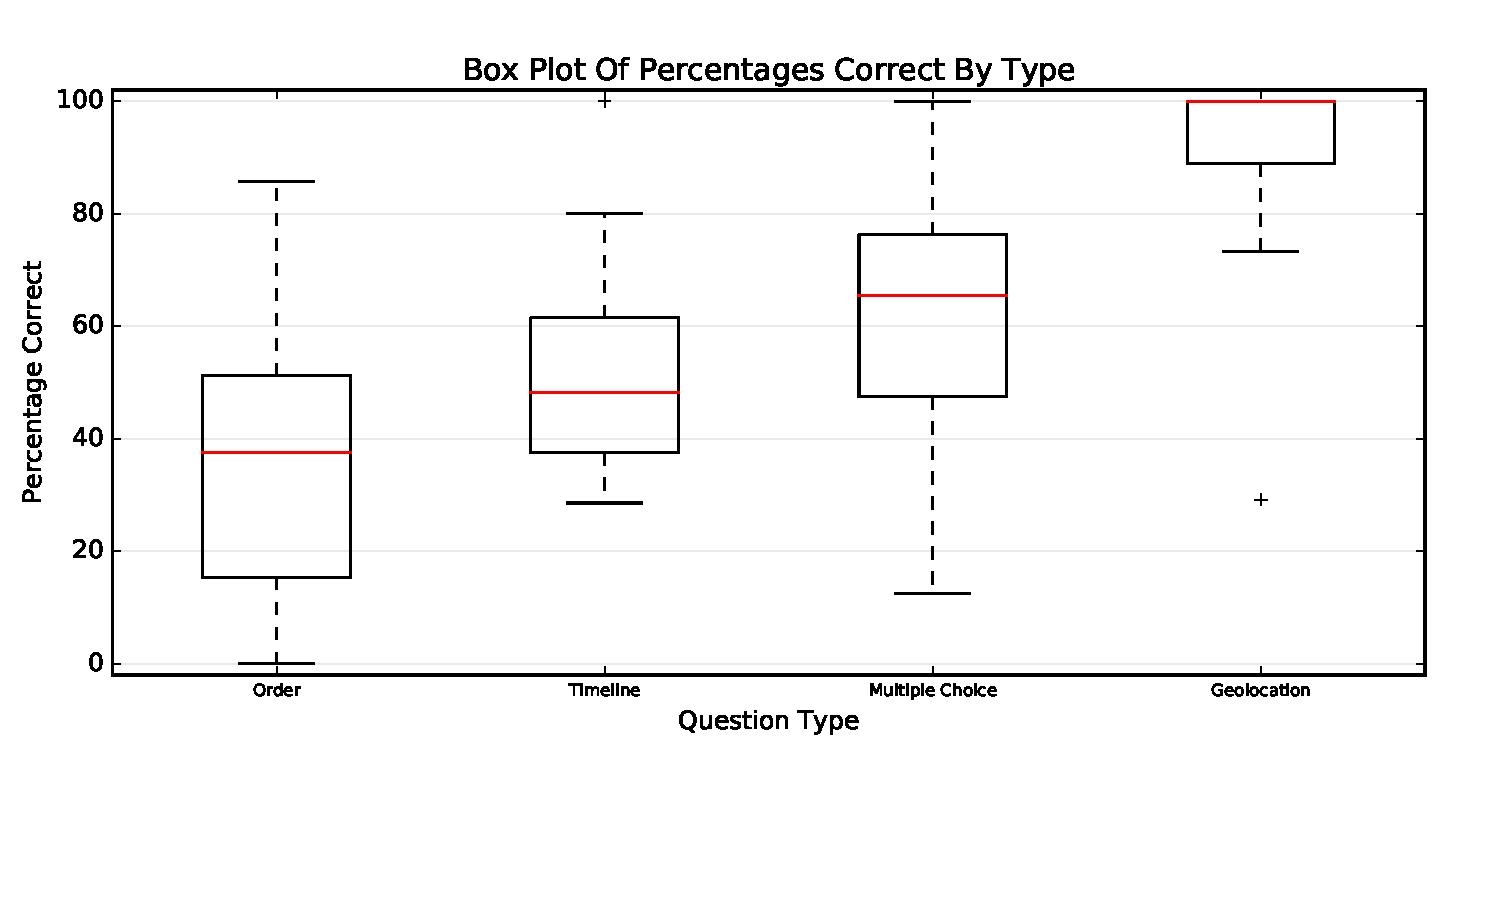
\includegraphics[width=4in]{images/pilot_1_boxplot.pdf}}
\caption{Percentages Correctly Answered Box Plots}
\label{fig:p1Boxes}
\end{figure}

\section{Time spent}
Figure \ref{fig:p1BoxesTime} shows that the time spent on timeline and multiple choice questions is pretty similar, it is a little higher for the multiple choice questions which can be explained by the higher number of possible answers. The ordering questions take more time probably because of the time taken for dragging the items. The most time is spent on the geolocation questions, it seems that there is some more thinking and the players might also be slowed down by the time taken to type their answer. However, it does not indicate that remembering a place is harder as the success rate on this kind of question is really high.
\begin{figure}
\centering
{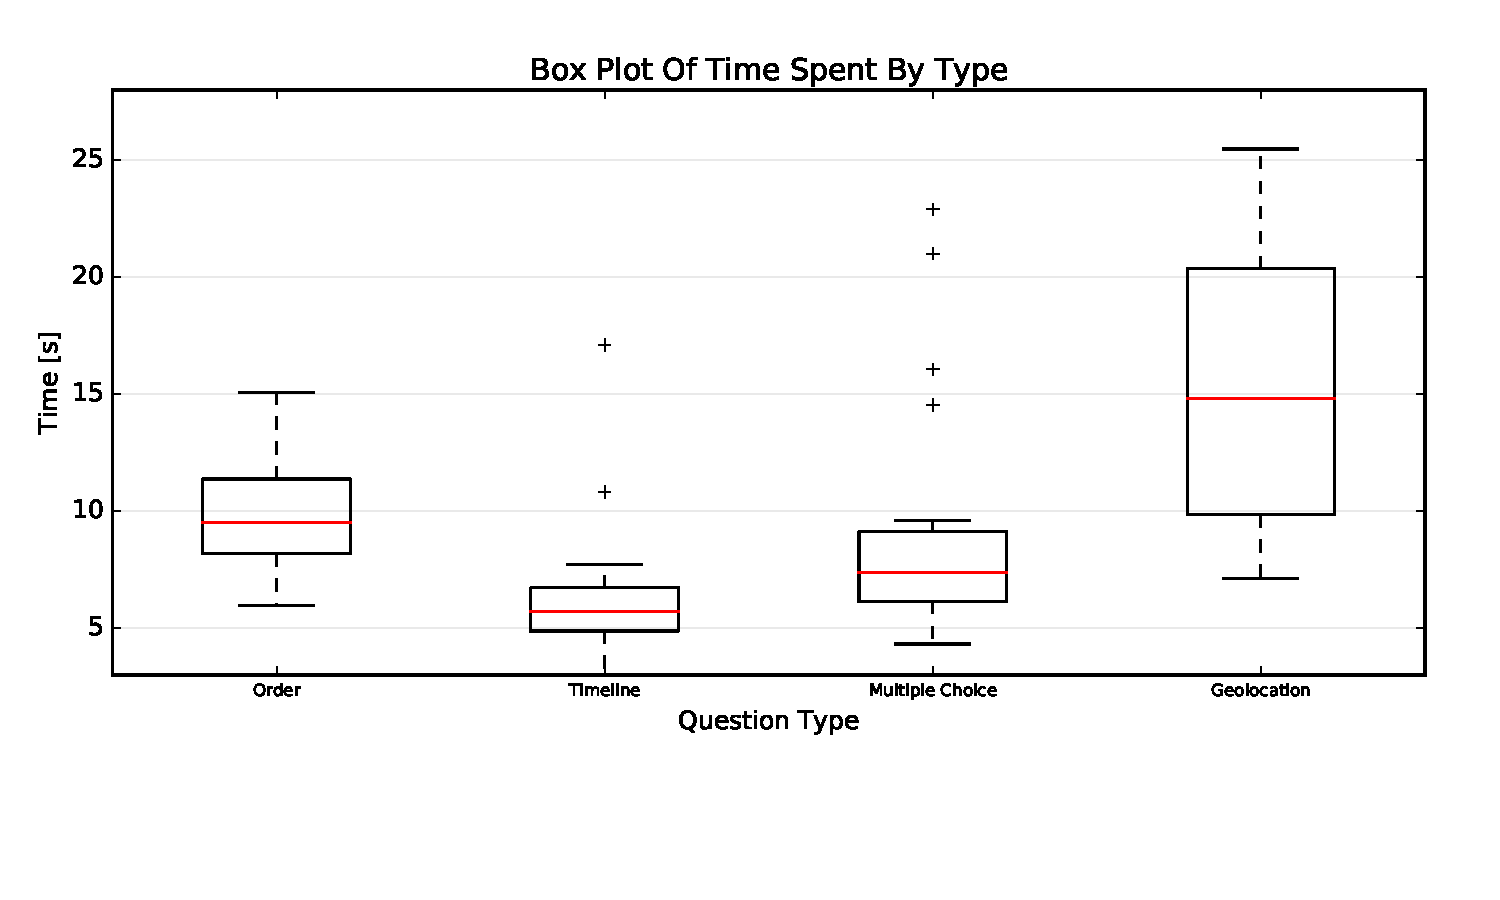
\includegraphics[width=4in]{images/pilot_1_boxplot_time.pdf}}
\caption{Box Plots Of Time Spent By Type}
\label{fig:p1BoxesTime}
\end{figure}

\section{Second pilot: on the influence of difficulty}
Following the same procedure, we asked friends and family to play the game. Over a bit more than a week, 40 different users played 155 games (on average 3.88 games per person) and answered 2517 questions. For this second pilot, we will perform the same general analysis and then dive in individual question types to try and see the impact of the difficulty.

\subsection{Selected Questions}
During this trial, people answered 546 order questions, 1022 timeline questions, 688 multiple choice questions and 261 geolocation questions. Of those questions 289 order questions, 592 timeline questions, 457 multiple choice questions and 223 geolocation questions were correct.\\
As for avoiding questions, 583 order questions, 1703 timeline questions, 815 multiple choice questions and 352 geolocation questions were avoided. This time we see an even clearer avoidance of timeline questions, a bit less avoidance than before for multiple choice questions and the geolocation questions are no longer picked as much. It is hard to interpret these results as the avoidance count does not take into account the board state at all which can have a huge influence on the result. It would be better to improve this measurement before trying to deduct anything. Figure \ref{fig:p2TotCorrectAvoid} shows a summary of those results.
\begin{figure}
\centering
{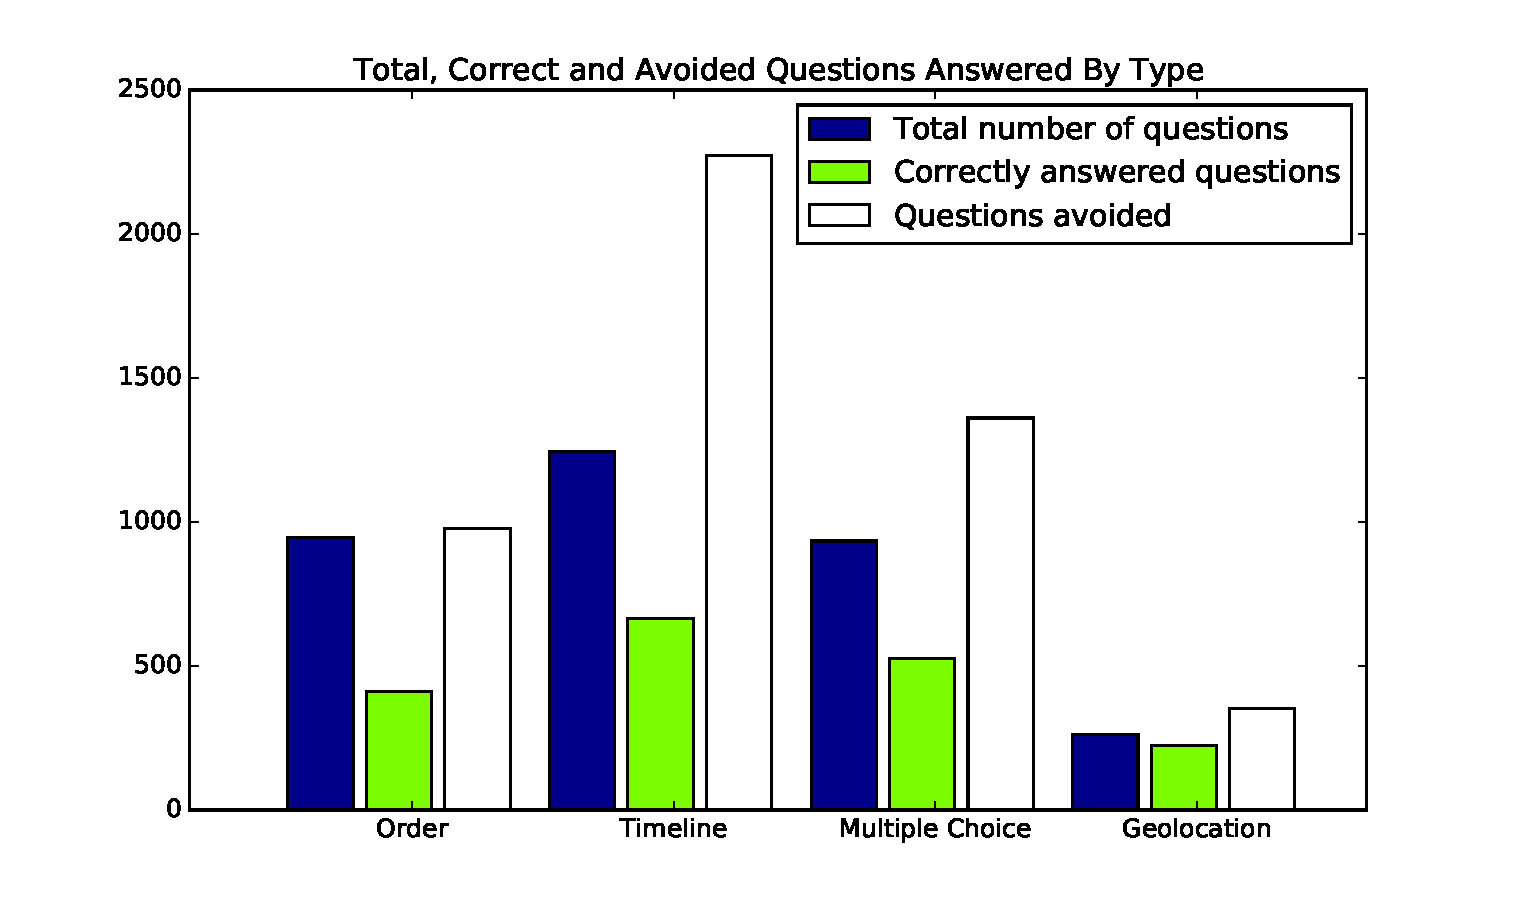
\includegraphics[width=4in]{images/pilot_2_selected_questions.pdf}}
\caption{Total, Correct and Avoided Questions Answered By Type}
\label{fig:p2TotCorrectAvoid}
\end{figure}
\subsection{Remembered Or Randomly Selected}\label{sec:p2remem}
On this pilot again we can again conclude that on average the people did not select their answer at random. The order questions were answered on average 48.63\% of the time correct, the timeline questions were answered correctly 56.78\% of the time and the multiple choice questions were answered correctly 66.69\% of the time. The really impressive result comes from geolocation questions, they were answered correctly a staggering 92.3\% of the time with a rather low standard deviation. Some more analysis on this particular result is done on section \ref{subsec:geolocissue}. Figure \ref{fig:p2Correct} shows an overview of these numbers.\\
As before a box plot (figure \ref{fig:p2Boxes}) can help us understand the data better. We see that this time, most of the people had between 42\% and 52\% success on the ordering questions, which is closer to the set goal as there are less people with a small amount of good answers. For timeline questions, most of the participant found themselves between 40\% and 67\% correct answers, this is a bit less close to the 50\% mark as the previous pilot which might mean that we are generating too easy questions. When it comes to multiple choice questions, there is a clear sign that our questions are too easy as most of the participants find themselves between 50\% and 84\%. Finally, geolocation answers where mostly comprised between 87\% and 100\% correct. This last results is a clear indicator that something is wrong with our geolocation questions.

\begin{figure}
\centering
{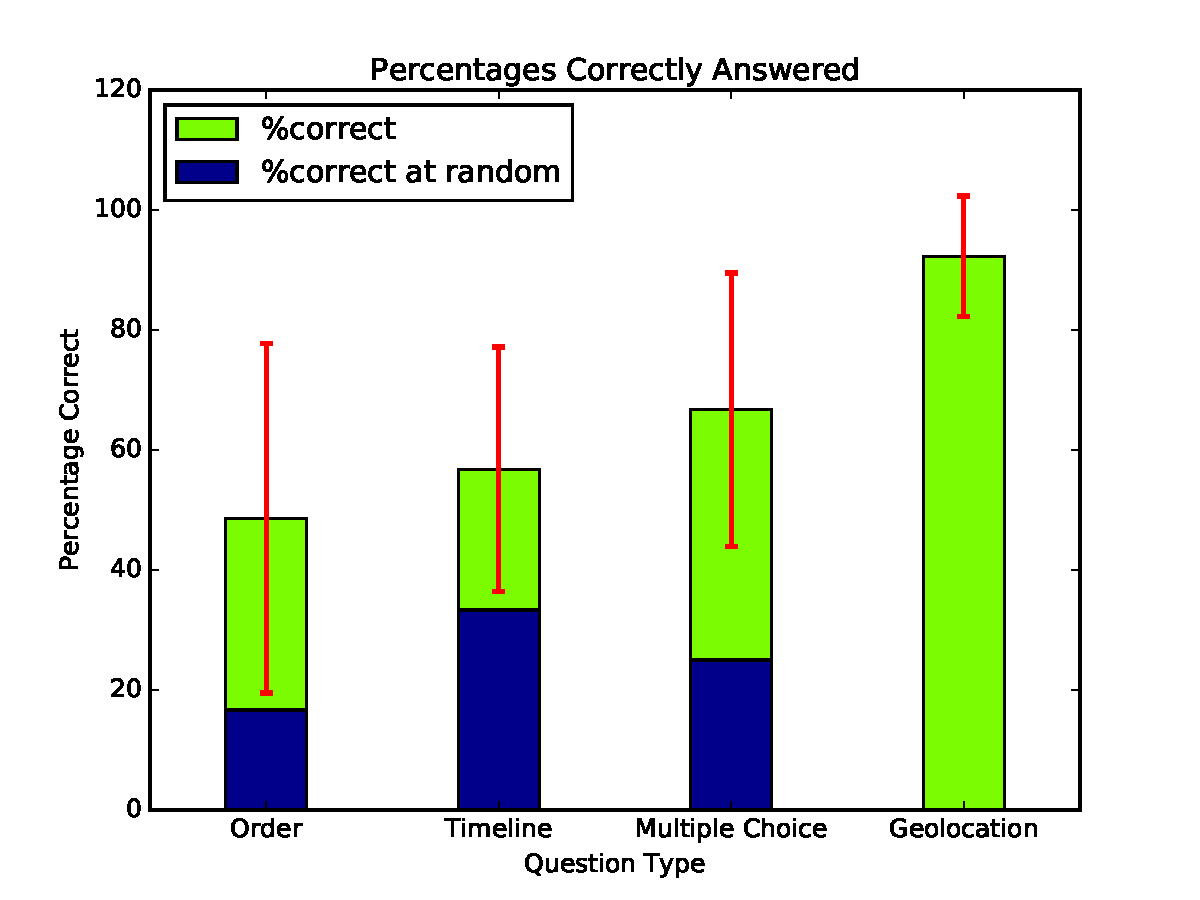
\includegraphics[width=4in]{images/pilot_2_correct.pdf}}
\caption{Percentages Correctly Answered}
\label{fig:p2Correct}
\end{figure}
\begin{figure}
\centering
{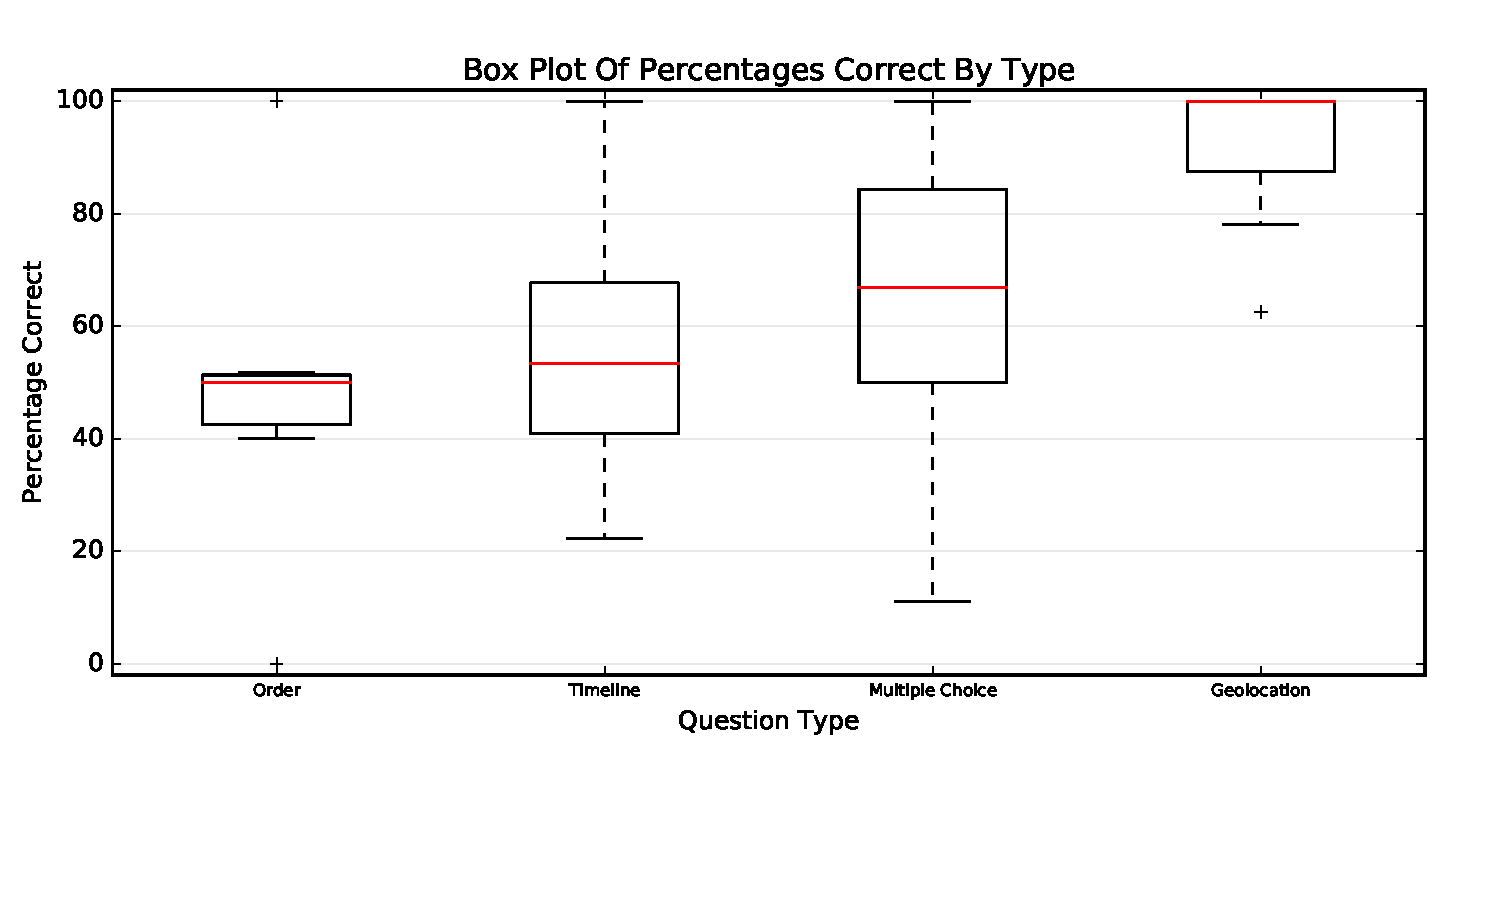
\includegraphics[width=4in]{images/pilot_2_boxplot.pdf}}
\caption{Percentages Correctly Answered Box Plots}
\label{fig:p2Boxes}
\end{figure}

\subsection{Ordering Questions}
The ordering questions results suggest that our question generating algorithm may be making slightly too harsh questions. The algorithm was designed to bring a user closer to a 50\% success rate over time, so the more a user play the closer they should get to 50\%. Figure \ref{fig:ordScatter} shows a scatter plot of the success rate of the players relative to their number of games played. The right half of the plot seems to suggest that the more games are played the closer to 50\% we get, but unfortunately the really small amount of data points does not permit to conclude anything definitively.

\begin{figure}
\centering
{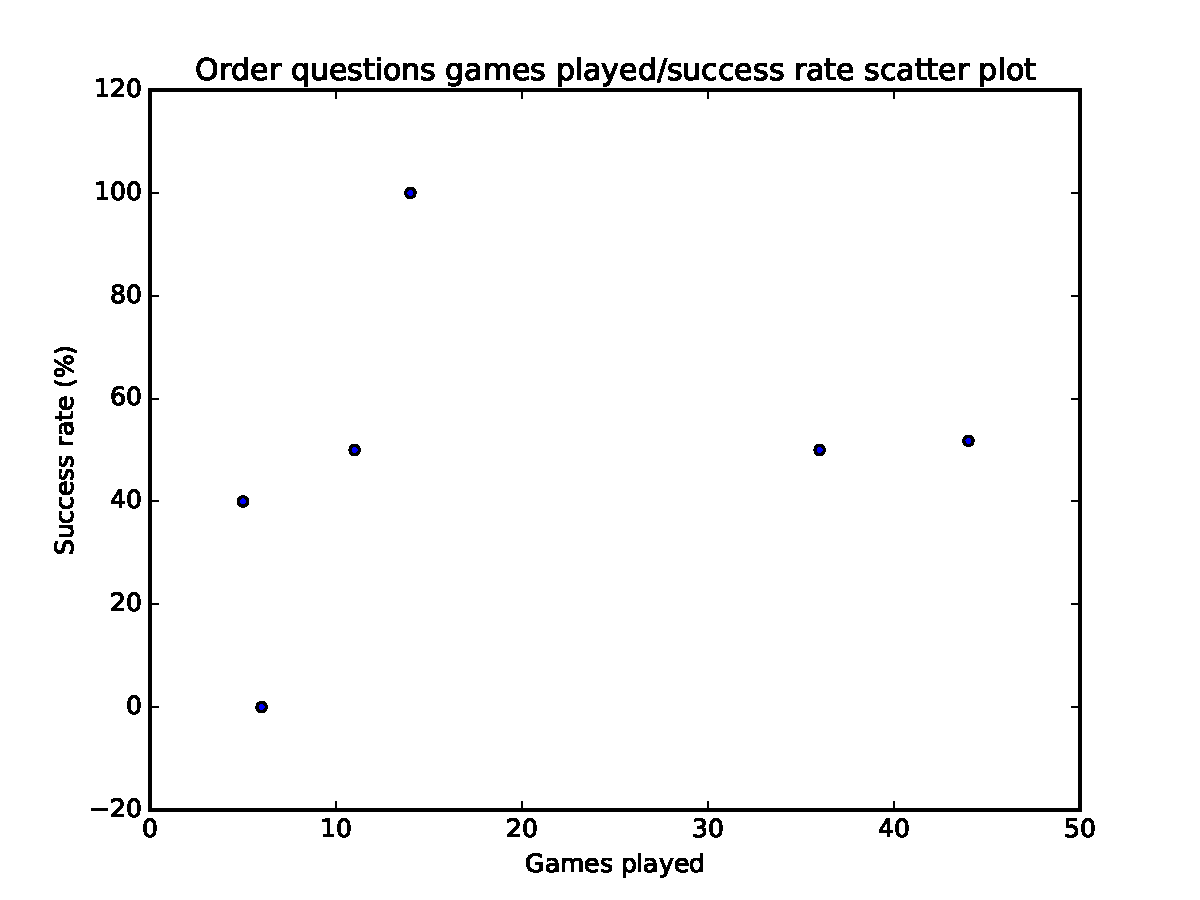
\includegraphics[width=4in]{images/order_scatter.pdf}}
\caption{Order questions games played/success rate scatter plot}
\label{fig:ordScatter}
\end{figure}

\subsection{Timeline Questions}
The box plot from section \ref{sec:p2remem} seems to suggest that the questions may be too easy but the range is quite large. The scatter plot on figure \ref{fig:timeScatter} shows that the people with less than 20 games had pretty random success rates on this question but the two people with more than thirty were around the 50\% success. While this is not sufficient to be certain of anything, it does suggest that for people playing a lot of games the result might be satisfying. The next step would then be to further investigate this possibility by having more people play a lot of games.\\
However this might also suggests that the questions are simply not difficult enough. One of the feedback was that the size of the proposed periods was not that small for events far in the past even for player with a high success rate.
\begin{figure}
\centering
{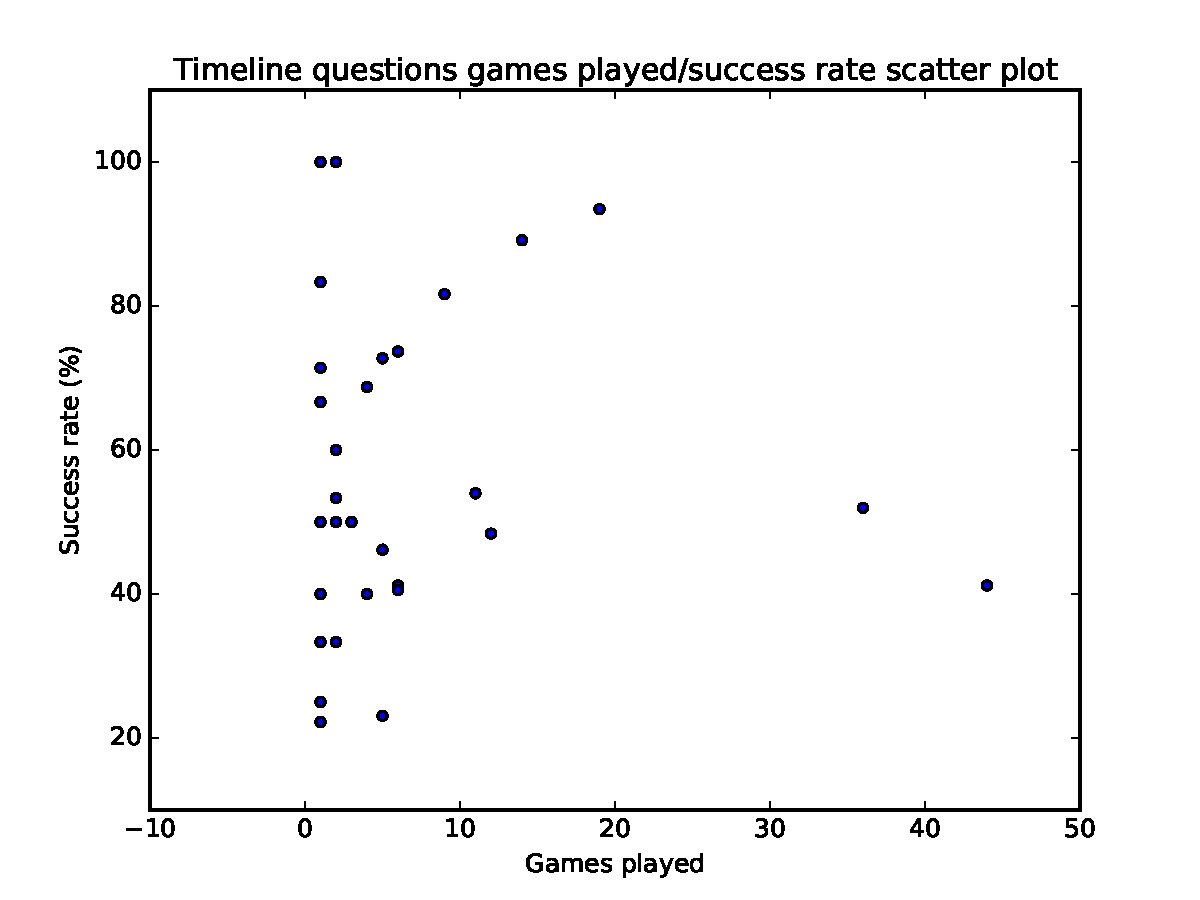
\includegraphics[width=4in]{images/timeline_scatter.pdf}}
\caption{Timeline questions games played/success rate scatter plot}
\label{fig:timeScatter}
\end{figure}

\subsection{Multiple Choice}
The box plot from section \ref{sec:p2remem} suggests that the questions are too easy. The scatter plot on figure \ref{fig:mcScatter} clearly shows that the questions are too easy. Most of the players have more than 50\% correct answers and nothing seems to indicate that it will drop as low as 50\% with a lot of games. The feedback also suggests the same. The "Which page did you like?" question is too easy as most of the time the non liked pages are unknown to the player. The questions about the reactions and comments offer more challenge but are still not hard enough.\\
To improve the situation, one should first gather more data with people playing more games while already making the multiple choice questions harder (being more aggressive with the difficulty parameters). Then, based on the new gathered data, a possible change of heuristic might be envisioned.
\begin{figure}
\centering
{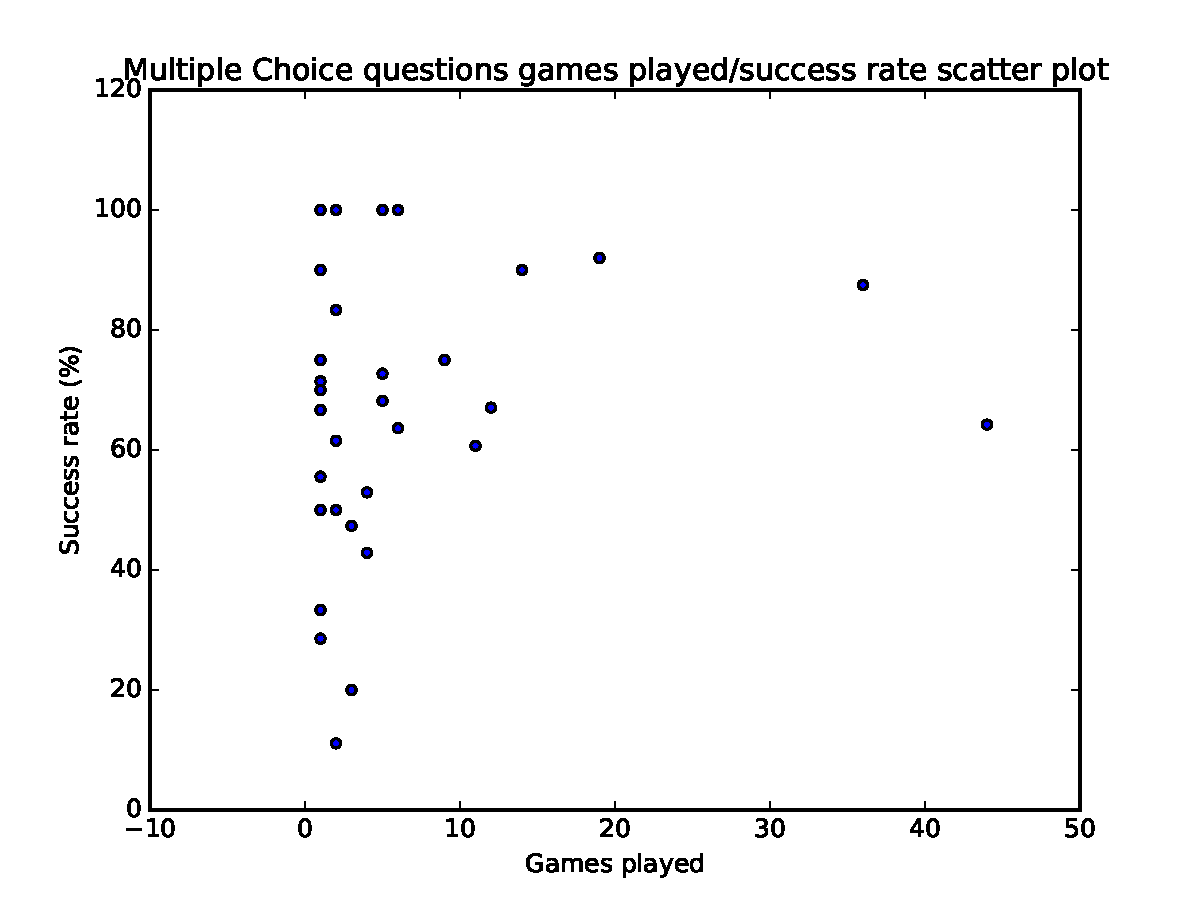
\includegraphics[width=4in]{images/mc_scatter.pdf}}
\caption{Multiple Choice questions games played/success rate scatter plot}
\label{fig:mcScatter}
\end{figure}
\subsection{Geolocation: the big problem}\label{subsec:geolocissue}
Let's first start with the scatter plot of figure \ref{fig:geoScatter}. It exhibits the same shape as the other scatter plots, only that nearly all the players have a success rate of more than 75\%. The problem of geolocation comes essentially from the amount of the geolocated posts we manage to get. First, as only a small portion of the posts are geolocated, they are by default more memorable than the others. Then, because players only have a few of them, the clustering algorithm often considers them all as being outliers and there according to the way we implemented those questions, they are always considered to be hard items. Therefore, a user will keep getting the same questions about the same places even though their success rate is already really high.\\
An other aspect that influences this situation is the tolerance we have to validate or not. Most of the time it suffices to remember in which city the post was geolocated, which is actually really easy even for places we do not know a lot about.

\begin{figure}
\centering
{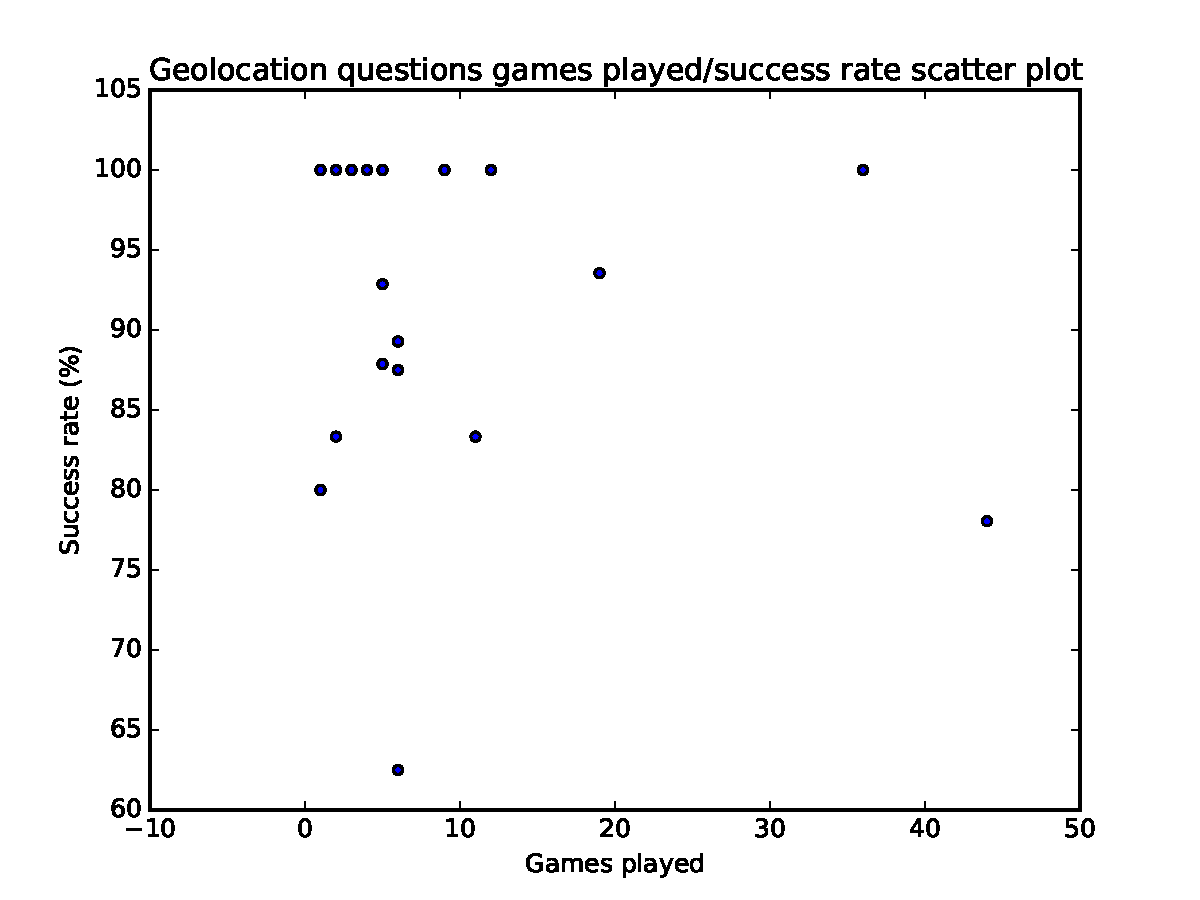
\includegraphics[width=4in]{images/geo_scatter.pdf}}
\caption{Geolocation questions games played/success rate scatter plot}
\label{fig:geoScatter}
\end{figure}

\subsection{What about the time spent?}
As suggested by figure \ref{fig:p2BoxesTime}, the timing results are pretty much the same as in the first pilot.
\begin{figure}
\centering
{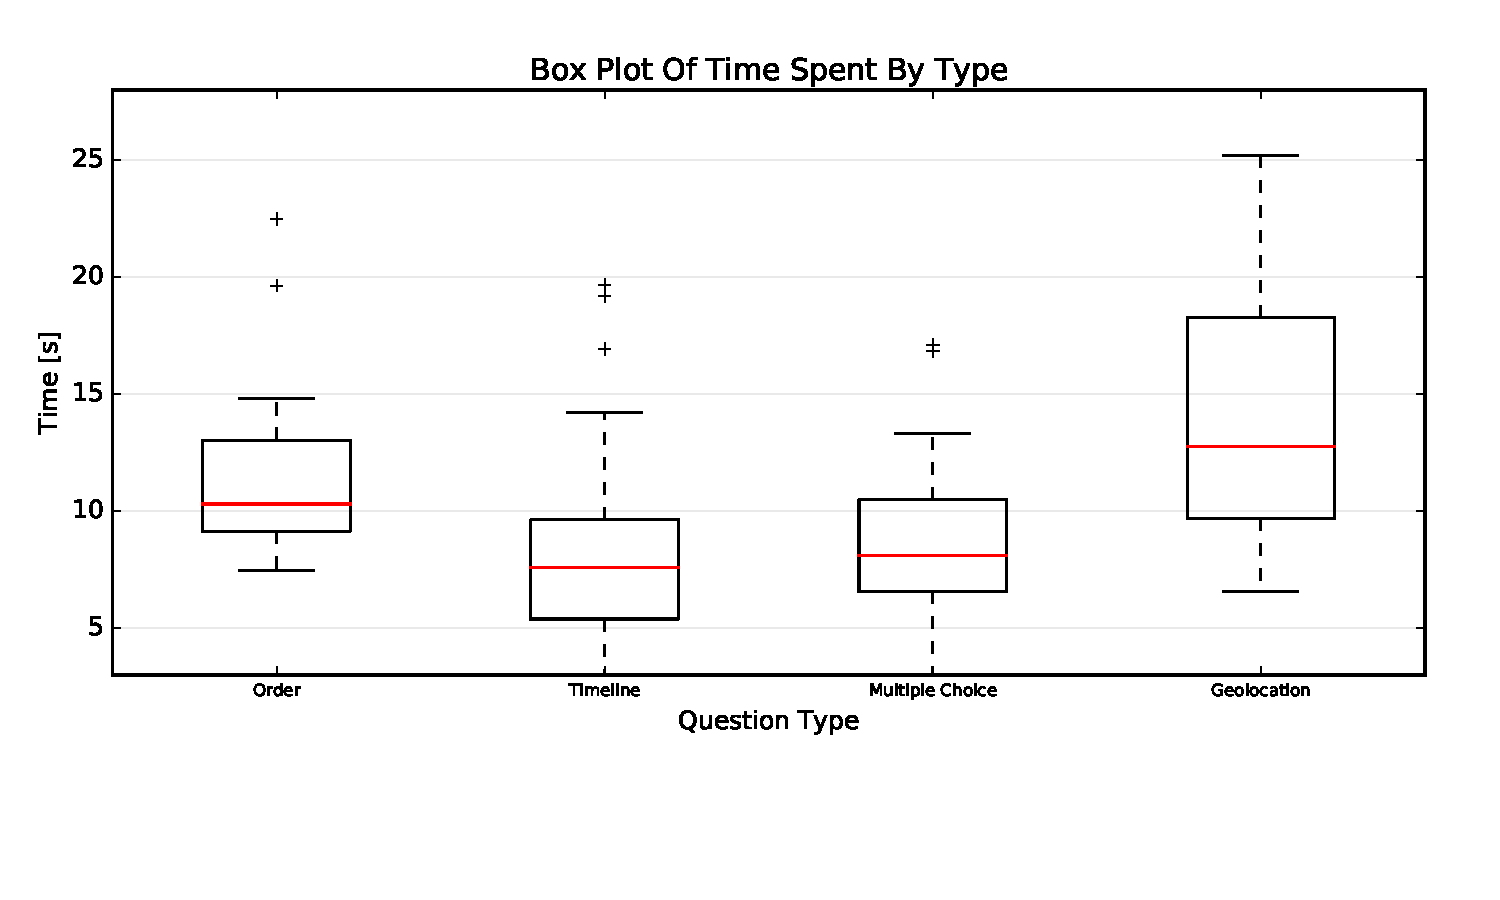
\includegraphics[width=4in]{images/pilot_2_boxplot_time.pdf}}
\caption{Box Plots Of Time Spent By Type}
\label{fig:p2BoxesTime}
\end{figure}

\subsection{More general feedback}
Based on some discussions
\begin{enumerate}
	\item The game is quite fun to play
	\item\label{void} Some of the questions are impossible to answer because of the lack of content on the post
	\item\label{lack} Some questions come back too often
\end{enumerate}
We cannot do a lot about item \ref{lack} because it is a direct consequence of the lack of facebook activity of those users. But item \ref{void} could be worked on. At the moment the techniques we use to filter posts with no content simply involved not using posts with absolutely no data, we could improve on this by analyzing the text and trying to determine if its content contains some interesting information or just some random rambling. This can be a quite involved task but we believe this could be done in the future.\\
A similar feedback was sometimes made about the questions involving the sharing of a link: some posts just have the link and being presented with just the link is often not enough to answer the question. This is a different issue and can be addressed by using Facebook Graph API which allows us to request more information about a post's attachments which could give us the extra information we need to generate better link questions.